\documentclass[12pt]{article}
 
\newenvironment{sol}[1][Solution]{\begin{trivlist}\item[\hskip\labelsep {\bfseries #1:}]}{\end{trivlist}}
\usepackage{minted}
%\usemintedstyle{perldoc}
\usemintedstyle{vs}
\usepackage{graphicx}
\graphicspath{./}

\usepackage[margin=1in]{geometry} 
\usepackage{amsmath,amsthm,amssymb}
\usepackage{times,url}
\usepackage{tikz}
\usepackage{enumerate}
\begin{document}
\renewcommand{\qedsymbol}{\filledbox}
\begin{center}
    \textbf{CS 5/7350 - Test\#1} \\
    \textbf{September 29, 2021}
%replace X with the appropriate number
\end{center}
\begin{flushright}
Name: \underline{Bingying Liang }\\
ID:  \underline{\ \ \ \ \ 48999397 \ \ \ \ \ }
\end{flushright}
\begin{enumerate}
    \item \ [6 pts] Define the following Terms as succinctly as possible:
    \begin{enumerate}
        \item Algorithm
        \begin{sol}
        A step-by-step procedure for solving a problem in a finite amount of time. 
        \end{sol}
        \item Big Omega
        \begin{sol}
        Is a possibly tight lower bound on a function
        \end{sol}
        \item Power Set 
        \begin{sol}
            A power set is the set of all subsets. For example: 
            \begin{align*}
                & S = {1, 2, 3} \\
                & P(S) = \{\{\}, {1},{2},{3},{1,2},{1,3},{2,3},{1,2,3}\}\\
                & |P(S)| = 2^s
            \end{align*}
            
        \end{sol}
        \item Compression
        \begin{sol}
            Compression means that we can use algorithms to reduce the number of bytes required to represent data and the amount of memory required to store images. 
        \end{sol}
        \item Entropy
        \begin{sol}
        In information theory, the entropy of a random variable is the average level of "information", "surprise", or "uncertainty" inherent to the variable's possible outcomes. Given a discrete random variable $X$,
$X$, which takes values in the alphabet $X$ and is distributed according to 
$p:X \rightarrow [0,1], \log_2\frac{1}{p(x)}$
        \end{sol}
        \item Merge Sort 
        \begin{sol}
        The Merge sort algorithm closely follows the divide-and-conquer method. In each step, it sorts a subarray $A[p:r]$, starting with the entire array $A[1:n]$ and recursing down to smaller and smaller subarrays.
        \end{sol}
    \end{enumerate}

    \item \ [7 pts] Argue that the problem, S, of sorting an unsorted array of integers of length greater than 100 elements is at least as hard - and maybe even harder - than the problem, L, of finding the ten largest elements of the same unsorted array of integers
    \begin{sol}
    The solution of problem can used to solve problem L, problem L can use the sorted array to find the ten largest elements. Therefore, problem S is at least as hard and maybe even harder than the problem L.\\
    \textcolor{red}{Since we can use a solver for problem S to solve problem L by sorting the array and then printing the last ten elements, Problem S must be just as hard or possibly harder than Problem L.}
    \end{sol}

    \item \ [8 pts] A tree has the following In-Order and Pre-Order traversals. Draw the tree and give the Post order traversal \\ 
    \begin{center}
        In Order: T M A Z P B L Q F N \\
Pre Order: L Z M T A P B Q N F
    \end{center}
    \begin{sol}
        T A M B P Z F N Q L
        \begin{center}
            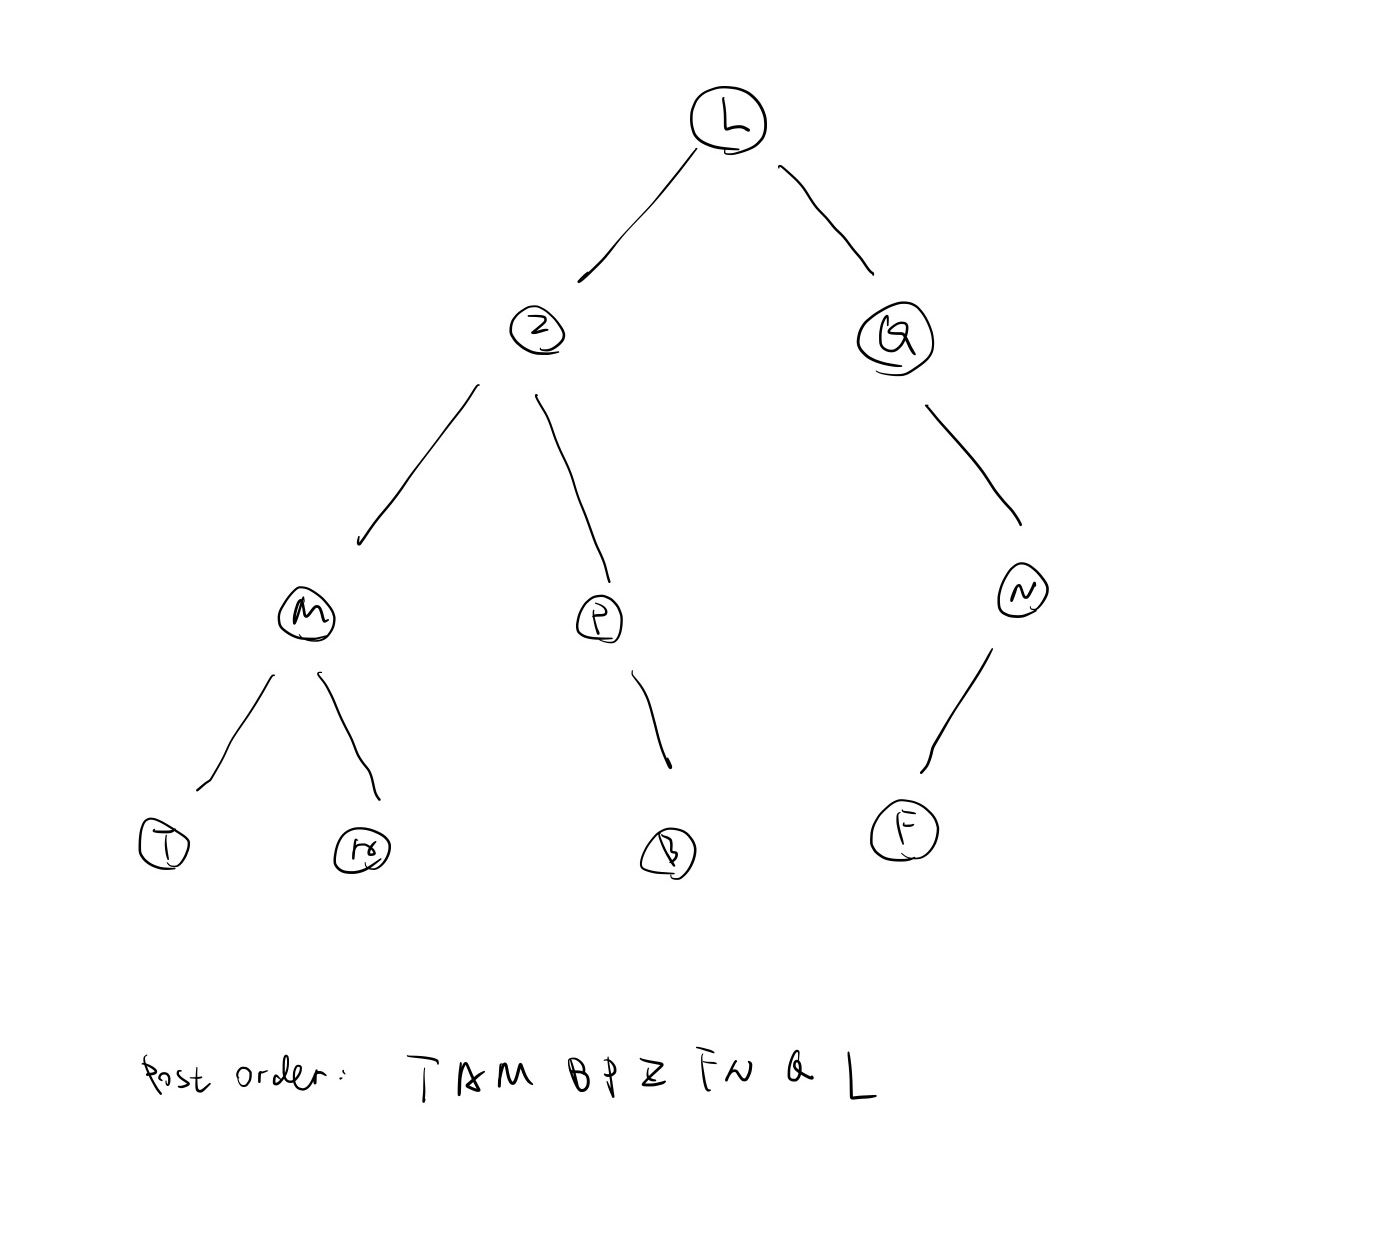
\includegraphics[width = 0.9\textwidth]{p1.jpg}
        \end{center}
    \end{sol}
    \item \ [7 pts] Using $n_0$ equal to 10, show that $f(n) = 8n^2 + 5n + 1 $ is $O(n^3)$.
    \begin{sol}
    \begin{align*}
        &O(g(n)) = \{f(n): \text{ there exist positive constants } c \text{ and } n_0 \text{ such that } \\
        & \ \ \ \ \ \ \ \ \ \ \ \ \ \ \ \ \ \ \ \ \ \ 0 \leq f(n) \leq cg(n) \text{ for all } n \geq n_0 \} \\
        & Assume \ n_0 = 10, g(n) = n^3 \\ 
        & 0 \leq 8n^3 + 5n + 1 \leq cn^3 \\
        & 8+\frac{5}{n^2} + \frac{1}{n^3} \leq c \\
        & if \ c = 80, n = 10\\
        & 8+\frac{5}{10^2} + \frac{1}{10^3} \leq 80\\
        & \therefore \text{ there exist positive constants } c \text{ and } n_0 \text{ such that } 0 \leq f(n) \leq cg(n) \text{ for all } n \geq n_0 \\
        & \therefore f(n) = 8n^2 + 5n + 1 \ is \ O(n^3)
    \end{align*}
    
    \end{sol}

    \item \ [8 pts] You run different programs for various values of “n” and create 4 tables of the runtimes. Give the Asymptotic bounds that each of the tables support?
        \begin{center}
            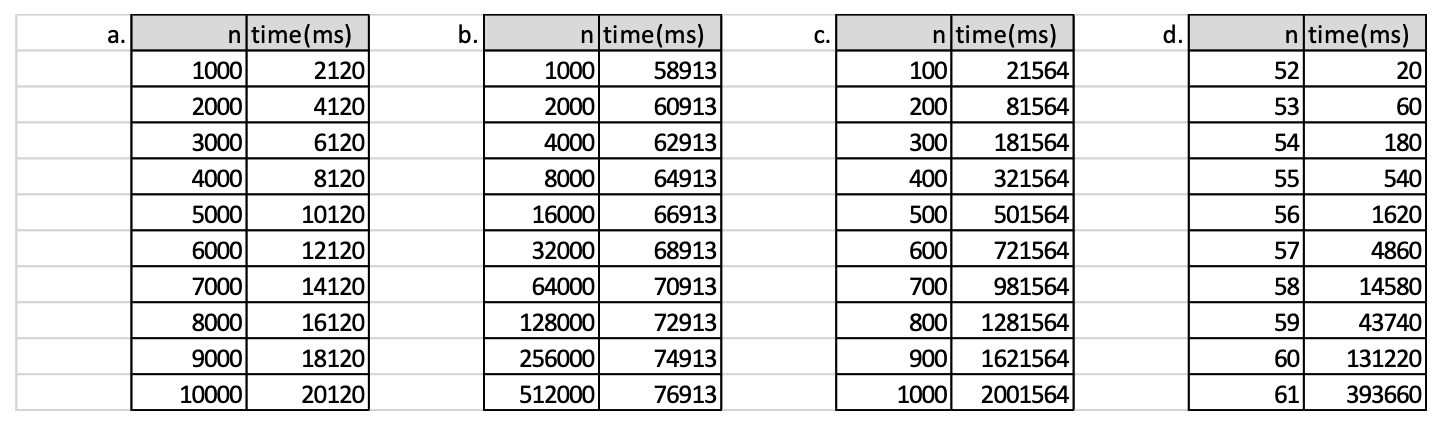
\includegraphics[width = 0.9\textwidth]{p2.png}
        \end{center}
        \begin{enumerate}
            \item $\Theta(n)$
            \item \textcolor{red}{$\Theta(logn)$}
            \begin{sol}
            \begin{align*}
                & \frac{\log_2(2000)}{\log_2(1000)} = \log_2(\farc{2000}{1000}) = \log_2(2) =1 \\
                & \frac{60913}{58913} = 1.033948365 \approx 1 
            \end{align*}
            \end{sol}
            \item $\Theta(n^2)$
            \item $\Theta(3^n)$
        \end{enumerate}


    \item \ [8 pts] Answer the following Questions:
    \begin{enumerate}
        \item Given that $M > 100 $ and $7^{31121} \bmod M = 8$; Find $7^{31122} \bmod M = $
        \begin{sol}
        56
        \begin{align*}
            & 7^{31122} \bmod M = 7^{31121+1} \bmod M = (7^{31121} \bmod 7) \times (7 \bmod M) = 8 \times 7 = 56
        \end{align*}
        \end{sol}

        \item How much entropy does an entire message with 40A’s and 60 B’s have?
        \begin{sol}
        \begin{align*}
            & p_A = \frac{40}{100}= \frac{2}{5}, p_B = \frac{60}{100} = \frac{3}{5} \\
            & = 40 \times \log_2(\frac{1}{p_A}) + 60 \times \log_2(\frac{1}{p_B})\\
            & = 40 \times 1.321928095 + 60 \times 0.736965594 \\
            & = 52.8771238+44.21793565 = 97.09505945 \approx 97.1 \ bits
        \end{align*}
        \end{sol}

        \item How much entropy does an entire message with 50A’s and 50 B’s have? 
        \begin{sol}
            \begin{align*}
            & p_A = \frac{50}{100}= \frac{1}{2}, p_B = \frac{50}{100} = \frac{1}{2} \\
            & = 50 \times \log_2(\frac{1}{p_A}) + 50 \times \log_2(\frac{1}{p_B})\\
            & = 100 \ bits
            \end{align*}
        \end{sol}

        \item Compute $(-\frac{1}{4}) \bmod 11 = $
        \begin{sol}
        \begin{align*}
            & (-\frac{1}{4} \times (-4)) \bmod 11 = 1 \bmod 11 = 1 \\
            & (-4) \times 8 \bmod 11 = -32 \bmod 11 = 1 \\
            & (-\frac{1}{4}) \bmod 11 = 8
        \end{align*}
        \end{sol}
    \end{enumerate}

    \item \ [8 pts] Consider a method of encoding a string where instead of using regular bits that take on values of 0 or 1, you use “ternary bits” with values 0, 1, or 2. For the following message:
    \begin{align*}
        \text{30 A’s, 14 B’s, 10 C's, 9 D's, 7 E's, 4 F's, 2 G's, 1 H and 1 K.}
    \end{align*}
    \begin{enumerate}
        \item How many of these ternary bits are in the entire message if each symbol is encoded with 2 of these “ternary bits” like this: A = 00; B = 01; C = 02; D = 10; E = 11; F = 12; G = 20; H = 21; K = 22
        \begin{sol}
        \begin{align*}
            (30 + 14 + 10 + 9 + 7 + 4 + 2 +1 +1) \times 2= 78 \times 2 = 156 \ bits
        \end{align*}
        \end{sol}

        \item Draw the tree and create a Huffman encoding of the ternary bits for each symbol:

        \item How many “ternary bits" are in the entire ternary Huffman coded message?
        \begin{sol}
        \hspace*{\fill}\\
        (b)(c)
        \begin{center}
            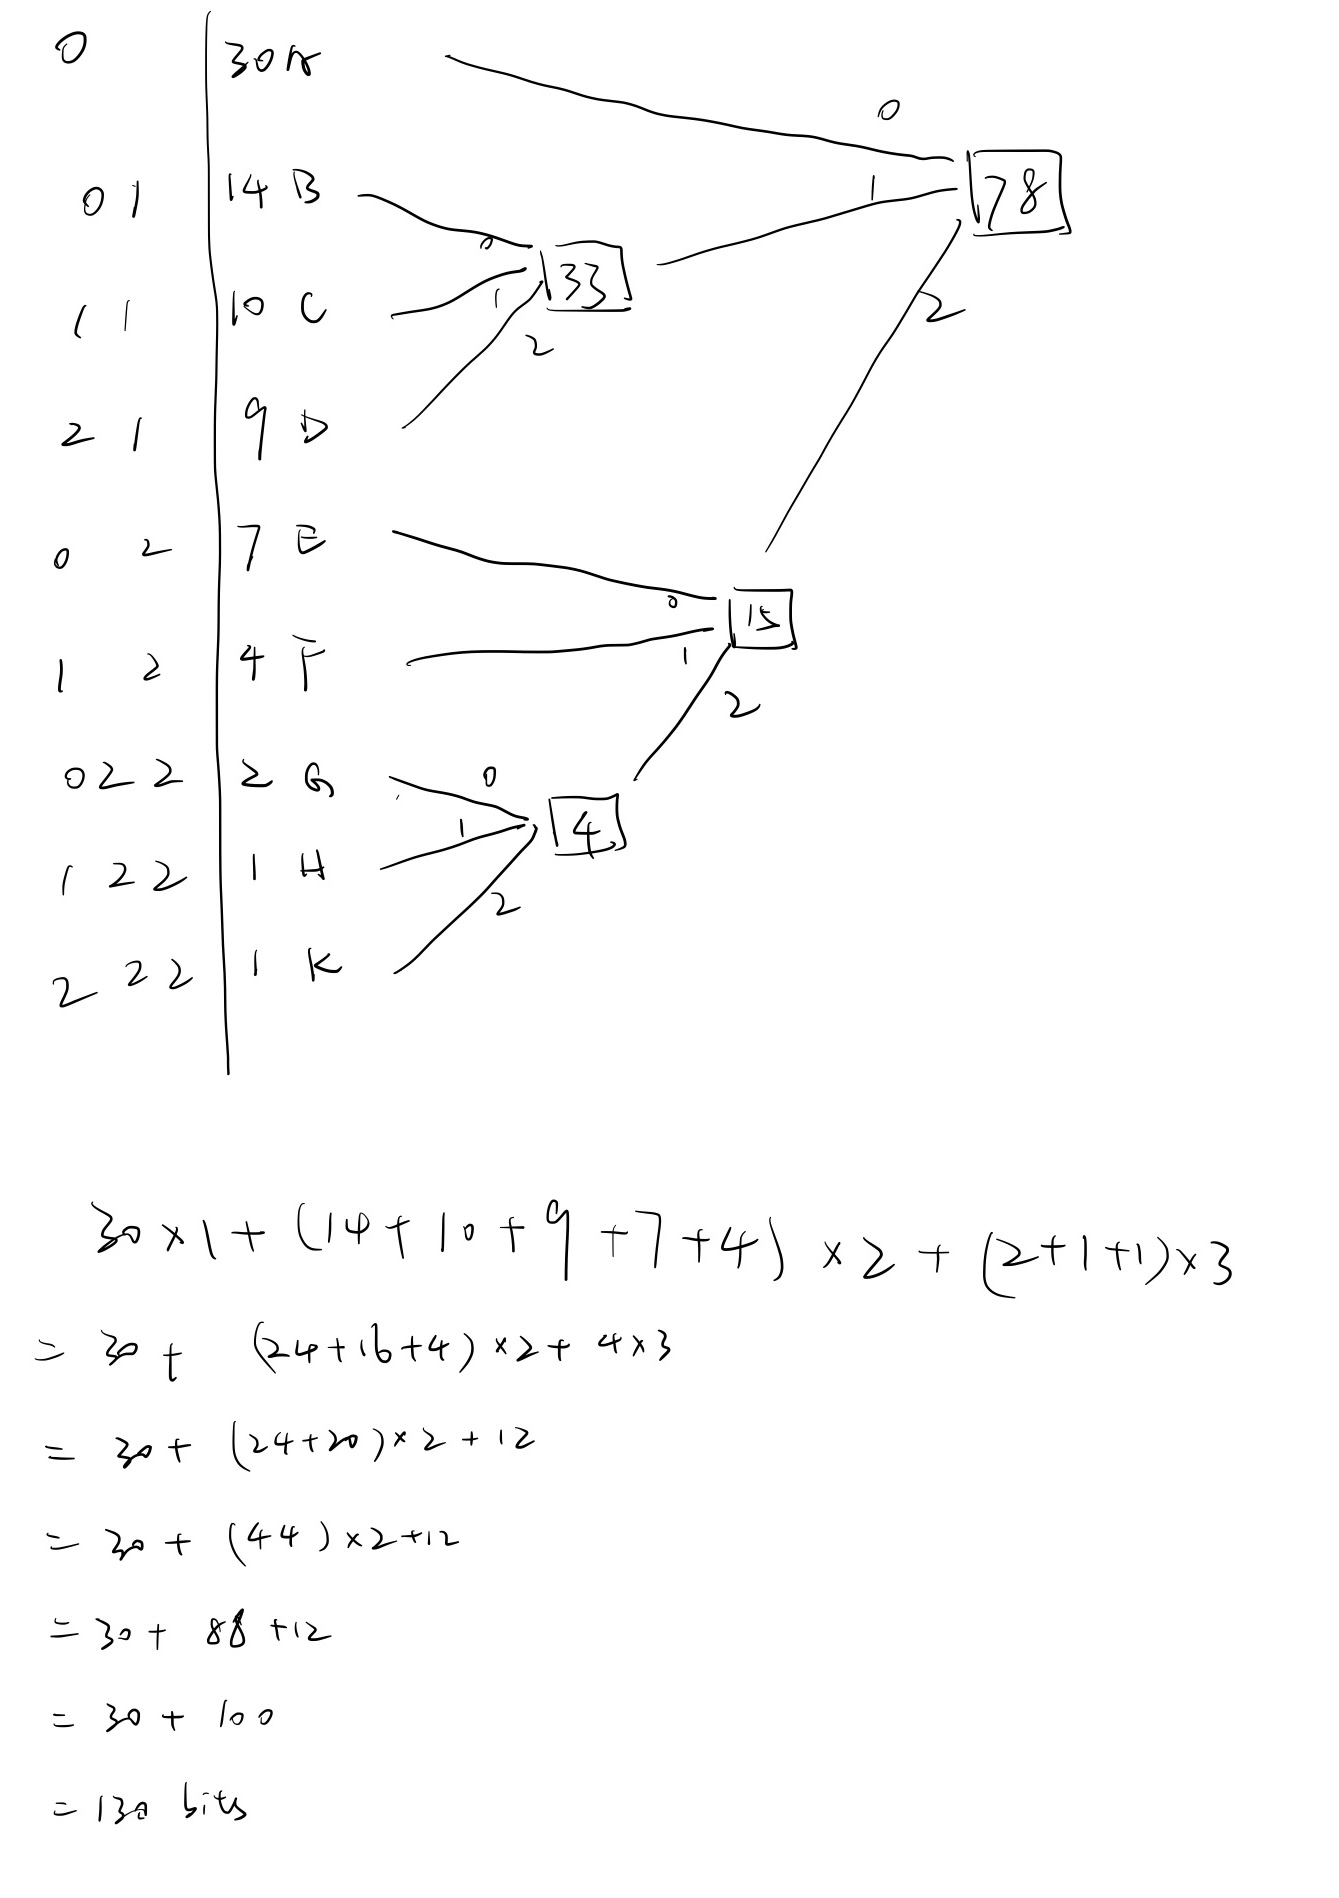
\includegraphics[width = 0.9\textwidth]{p3.jpg}
        \end{center}
        \end{sol}
        
    \end{enumerate}



    \item \ [5 pts] Two people need to establish a secret key for encrypting communications. They agree to use a Diffie-Hellman key exchange with a modulus of 11 and decide on 2 as the base. Person A chooses a random value performs the appropriate computations and sends the value 6 to person B. Person B chooses a random value of 3 and performs the appropriate computations:
    \begin{enumerate}
        \item What is the value Person B sends to Person A
        \item What is the shared secret key between Person A and Person B
        \begin{sol}
        (a)(b)
        \begin{center}
            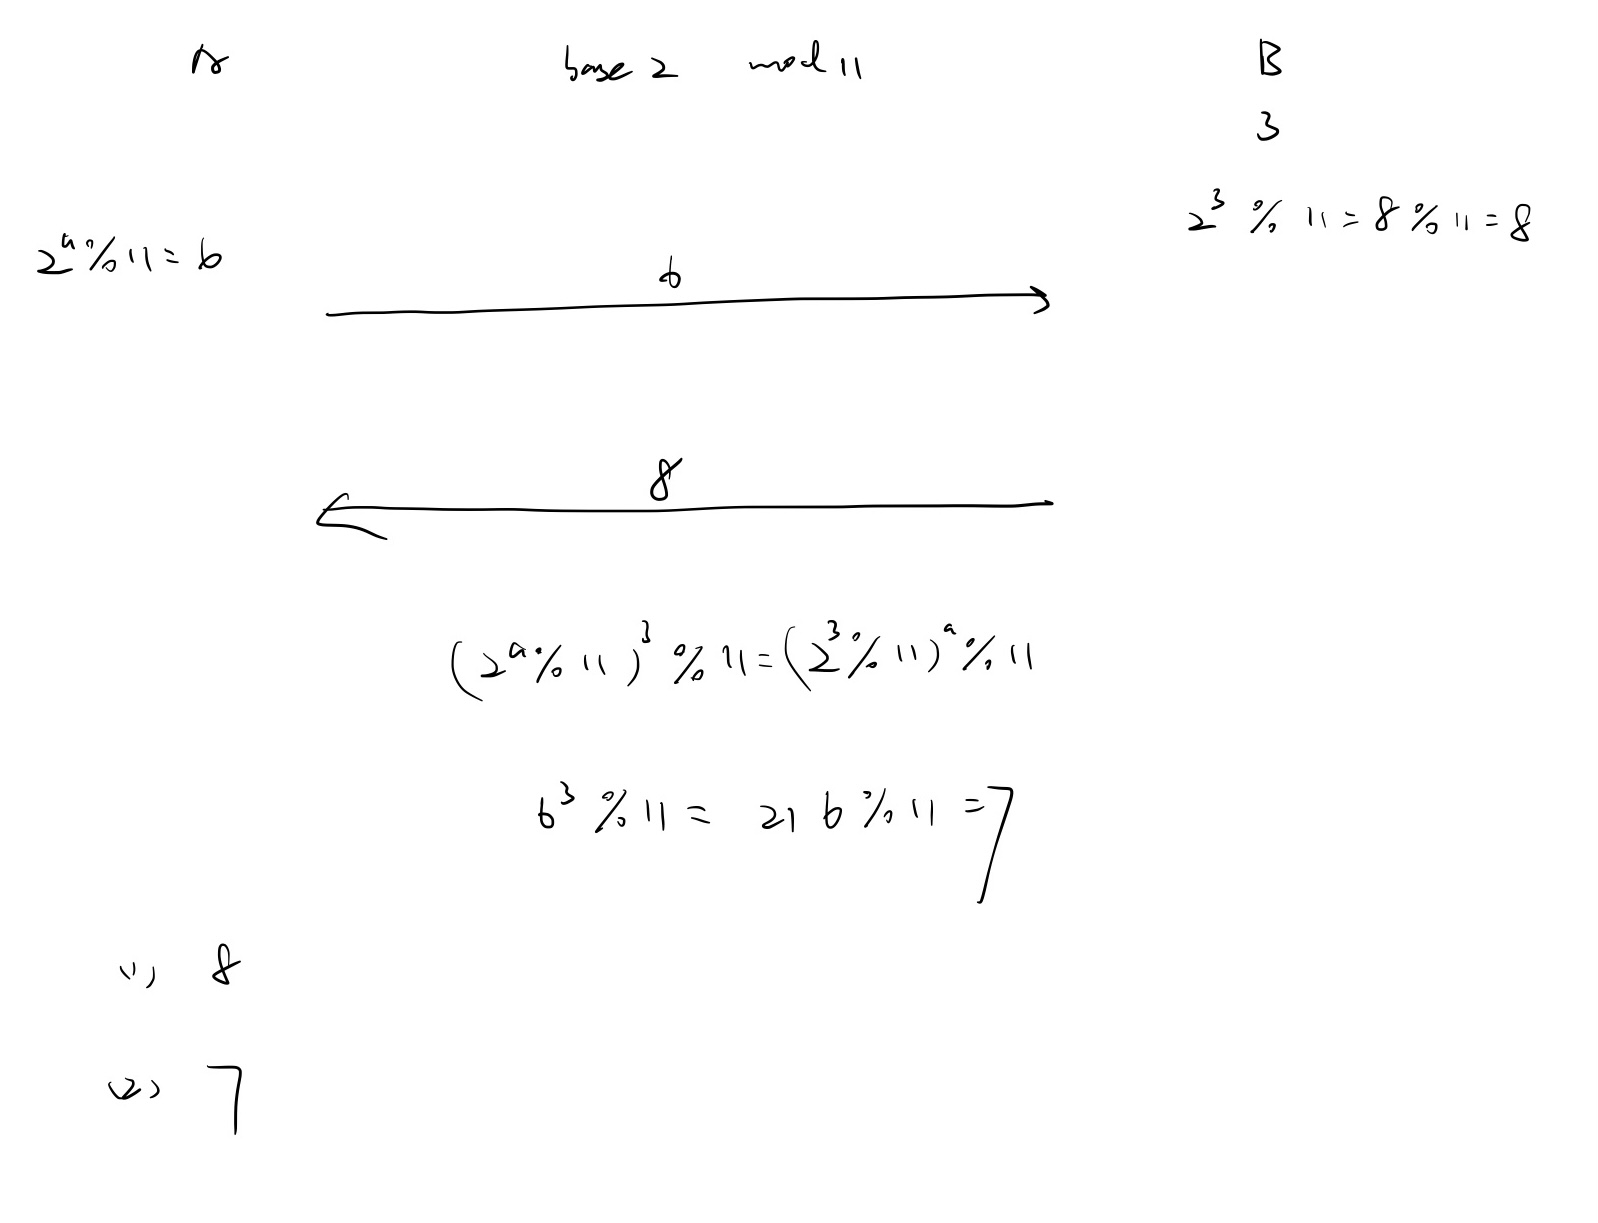
\includegraphics[width = 0.9\textwidth]{p4.jpg}
        \end{center}
        \end{sol}

    \end{enumerate}

    \item \ [10 pts] Consider two different algorithms that each solve a different problem.
    \begin{itemize}
        \item Implementation X solves Problem $P_x$ and Implementation X is $\Theta(n)$
        \item Implementation Y solves Problem $P_y$ and Implementation Y is $\Theta(2^n)$
    \end{itemize}
    Determine if each of these “Yes it is true”, “Maybe it is true but doesn’t have to be”, or “No it is not true”
        \begin{enumerate}
        \item Problem Px is harder than Problem Py: M
        \item Problem Py is harder than Problem Px: M
        \item Implementation X is harder than Implementation Y: N
        \item Problem X is $\Omega(n)$: \textcolor{red}{M} 
        \begin{sol}
            Because Implementation X is $\Theta(n)$, Problem X should be equal or less than that. Problem lower bound should be lower or equal than Implementation.
        \end{sol}
        \item Problem X is $\omega(n)$: N
        \textcolor{red}{\item Problem X is $O(n)$: Yes} %M
        \item Problem X is $o(n)$:\textcolor{red}{M} 
        \begin{sol}
        Problem x o(n) can be equal or smaller than $O(n)$, for example, the Problem $\Theta(\log n)$ and the $O(\log n)$ which is satisfied the lower bound should lower than Implementation.
        \end{sol}
        \item Implementation X is $\Omega(n)$:Y
        \item Implementation X is $\omega(n)$:N

    \end{enumerate}

    
    \item \ [8 pts] The graph below represents containers that are transported between these cities each day. You are determining the maximum flow from vertex S, Vancouver, to vertex T, Winnipeg, using the Ford-Fulkerson algorithm in the graph below.
        \begin{center}
            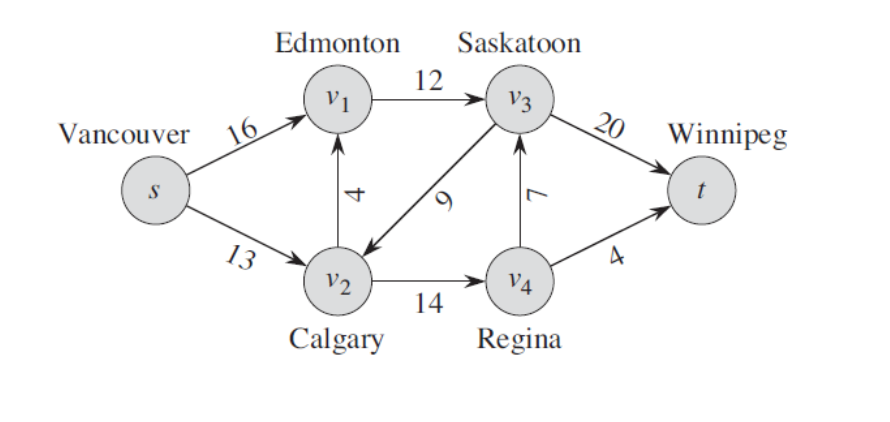
\includegraphics[width = 0.6\textwidth]{p5.png}
        \end{center}
        A Path Search finds the path $s \rightarrow v_2 \rightarrow v_1 \rightarrow v_3 \rightarrow t$
        \begin{enumerate}
            \item How much flow is in this path?
            \item What does the new graph look like after “removing” this flow

    \begin{sol}
        \begin{center}
            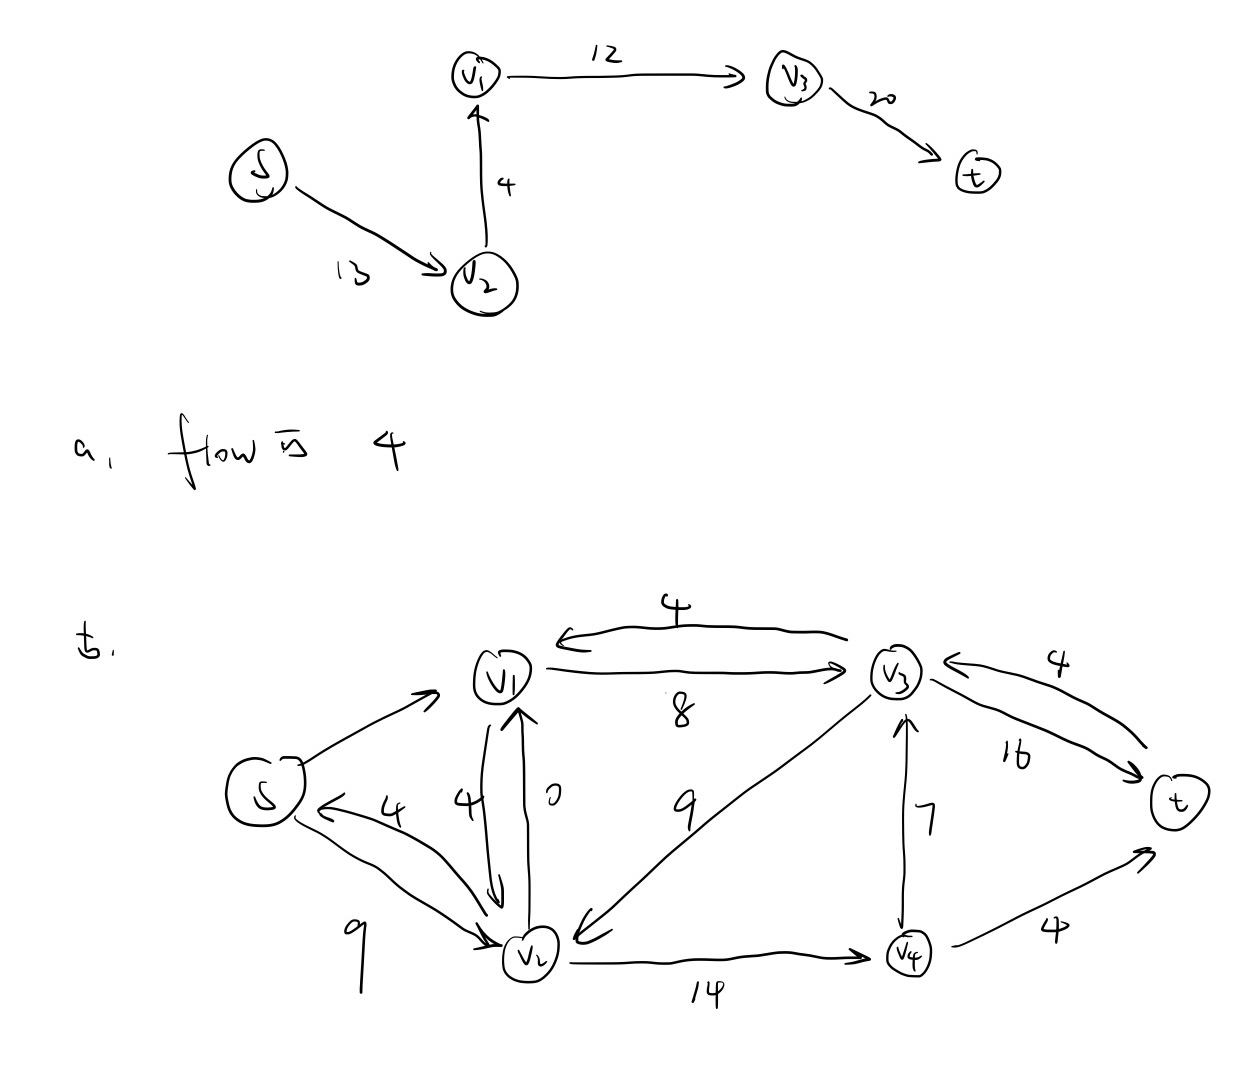
\includegraphics[width = 0.7\textwidth]{p6.jpg}
        \end{center}
        
    \end{sol}
    A Path Search now finds the path $s \rightarrow v_1 \rightarrow v_2 \rightarrow v_4 \rightarrow v_3 \rightarrow t$ on the new graph.
\item Is it possible to find this path?
\item If so, how much flow is in this path?
\item If so, what does the new graph look like after “removing” this flow?
        \begin{sol}
        \hspace*{\fill}\\
        \begin{center}
            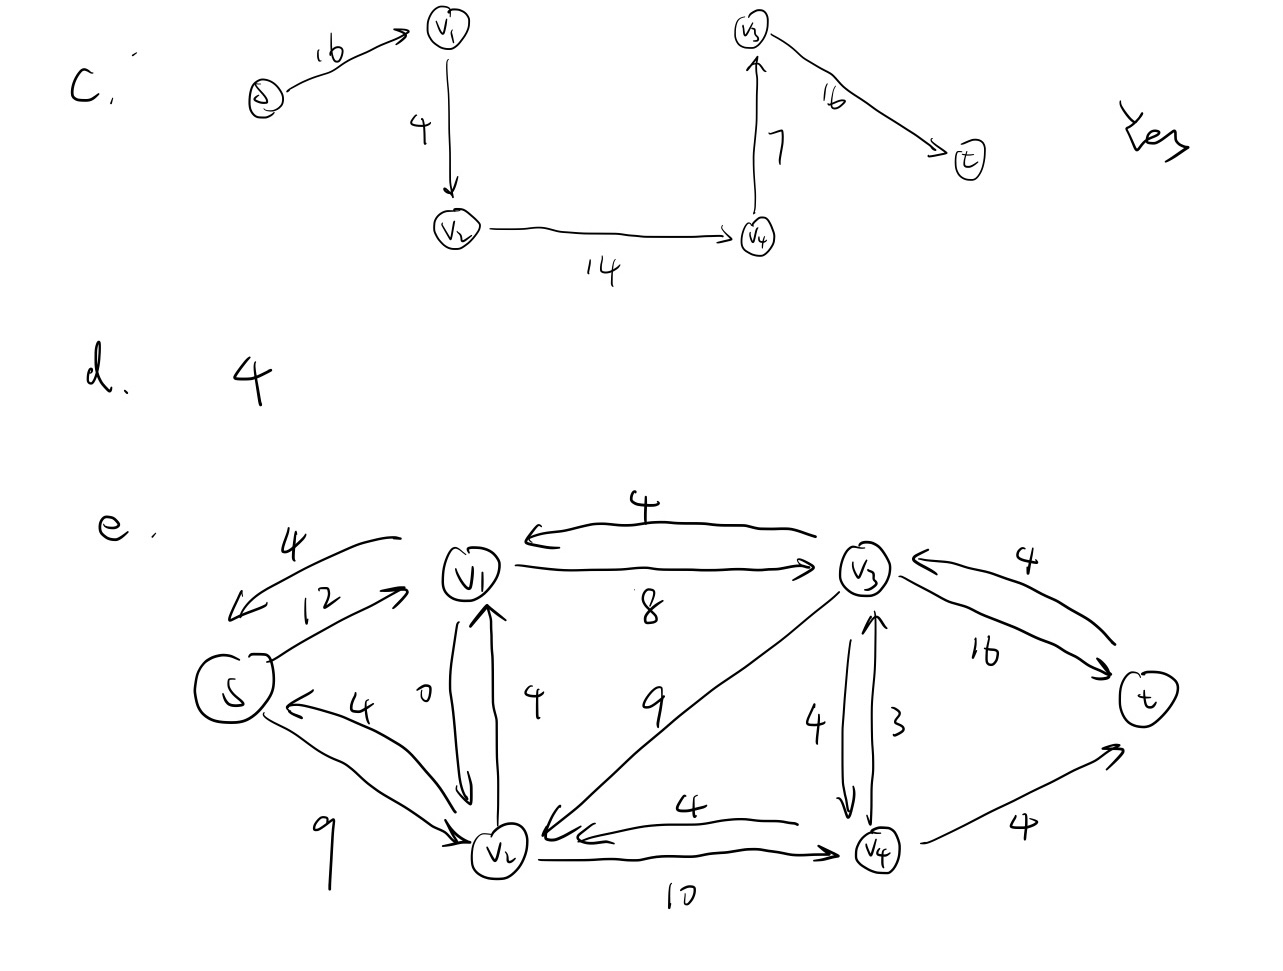
\includegraphics[width = 0.9\textwidth]{p7.jpg}
        \end{center}
        
    \end{sol}
        \end{enumerate}

    \item \ [10 pts] Answer the following questions.:
    \begin{enumerate}
        \item A program requires 6 seconds to process an input size of 80. If the running time is $\Theta(\sqrt{n})$ about how large of an input set could you process in 600s?
        \begin{sol}
        \begin{align*}
            \frac{\sqrt{n}}{\sqrt{80}} \times 6 = 600 \rightarrow n = 800000
        \end{align*}
        \end{sol}
        \item A program requires 5 DAYS to brute force attack a password of 50 bits. Since the running time is $\Theta(2^n)$ about how MANY YEARS would it take for the program to brute force attack a password of 512 bits?
        \begin{sol}
            \begin{align*}
                \frac{\frac{2^{512}}{2^{50}} \times 5}{365} \ years
            \end{align*}
        \end{sol}
        \item A program requires 5 DAYS to brute force attack a password of 50 bits. Since the running time is $\Theta(2^n)$ about how MANY DAYS would it take for the program to brute force attack a password of 512 bits if the running time were $\Theta(n^2)$ instead of exponential?
        \begin{sol}
            \begin{align*}
            \frac{512^2}{50^2} \times 5 = \frac{262144}{2500} \times 5 \approx 525 \ days
            \end{align*}
        \end{sol}
        \item A program requires 6 milliseconds to process an input size of 1000. If the running time is $\Theta(n^3)$ about how many seconds would it take to process an input size of 1 trillion items?
        \begin{sol}
            \begin{align*}
                \frac{(1 \times 10^{12})^3}{(1 \times 10^3)^3} \times 6 \times 10^{-3} = 6 \times 10^{24} \ seconds
            \end{align*}
        \end{sol}
        \item A program requires 6 milliseconds to process an input size of 1000. If the running time is $\Theta(n)$ about how long many seconds it take to process an input size of 1 trillion items?
        \begin{sol}
            \begin{align*}
                \frac{1 \times 10^{12}}{1 \times 10^3} \times 6 \times 10^{-3} = 6 \times 10^6 \ seconds
            \end{align*}
        \end{sol}



    \end{enumerate}

    \item \ [8 pts] Answer the following questions:
    \begin{enumerate}
        \item What is the weight of a minimum spanning tree for a complete graph with 10
vertices where all edges have a weight of 4?
        \begin{sol}
            $4(|V|-1) = 36$ 
        \end{sol}
        \item What is the weight of a minimum spanning tree for a cycle with 10 vertices where all edges have a weight of 4?
        \begin{sol}
            $4(|V|-1) = 36$
        \end{sol}
        \item A complete bi-partite graph $B_{j,k}$ is a graph which has J vertices in one partition and k vertices in another partition and all possible edges present between the partitions. For which values of j and k does a cycle exist that spans all the vertices?
        \begin{sol}
            \textcolor{red}{$j = k \ and \ j,k \geq 2$}
        \end{sol}
        \item What is the weight of a minimum spanning tree for a connected bi-partite graph Bj,k where all edges have a weight of 4?
        \begin{sol}
            $4(J+K-1)$
        \end{sol}

    \end{enumerate}


    \item \ \textcolor{red}{[7 pts] You live in city G. You want to know the cost to travel from city G to all other cities (A,B,C,D,E,F,H and I). The edges of the graph below represent the cost to travel the roads between various cities. If an edge doesn’t exist, then there is no road between those two cities.}
        \begin{center}
            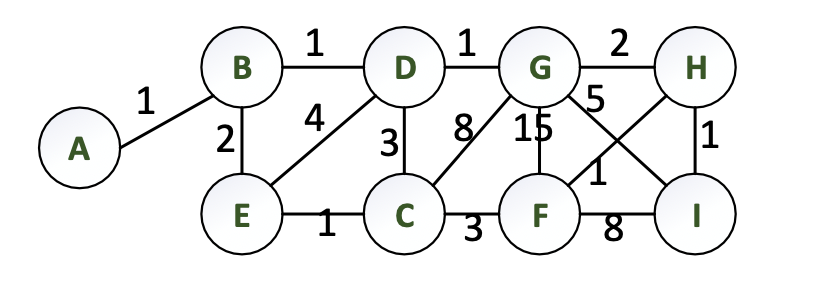
\includegraphics[width = 0.6\textwidth]{p8.png}
        \end{center}

        \begin{enumerate}
            \item What is the order in which you explore the cities using Dijkstra’s Single Source Shortest Path algorithm to find the cost from city G to all other cities in the graph?
            \item Write the cost to reach each city from City G by its vertex in the graph.
        \end{enumerate}
        \begin{sol}
                \hspace*{\fill}\\
                \begin{center}
            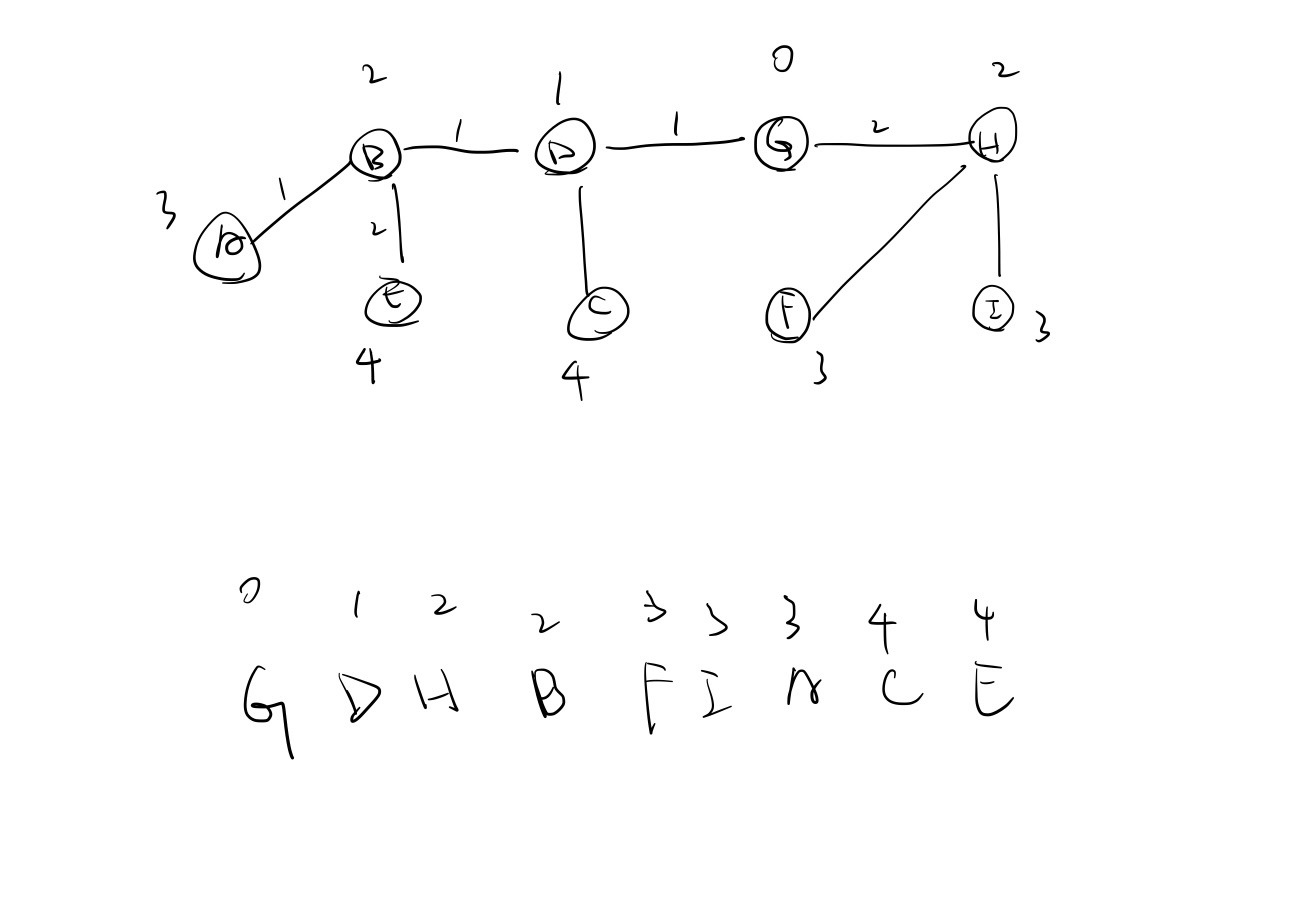
\includegraphics[width = 0.6\textwidth]{p9.jpg}
        \end{center}
        \end{sol}
        

\end{enumerate}
\end{document}
